\documentclass[a4paper,11pt,final]{article}
% Pour une impression recto verso, utilisez plutôt ce documentclass :
%\documentclass[a4paper,11pt,twoside,final]{article}

\usepackage[english,francais]{babel}
\usepackage[utf8]{inputenc}
\usepackage[T1]{fontenc}
\usepackage[pdftex]{graphicx}
\usepackage{setspace}
\usepackage{hyperref}
\usepackage[french]{varioref}
\usepackage{fancyhdr}
\usepackage{lastpage}
\usepackage{titlesec}
\usepackage[title,titletoc]{appendix}
\usepackage{rotating}
\usepackage{alltt}

\newcommand{\reporttitle}{Rapport de projet Infographie$\newline$Ace Attorney 3D}     % Titre
\newcommand{\reportauthor}{Vincent \textsc{Metton}, Grégoire \textsc{Pommier}} % Auteur
\newcommand{\reportsubject}{}  % Sujet
\newcommand{\HRule}{\rule{\linewidth}{0.5mm}}
\setlength{\parskip}{1ex} % Espace entre les paragraphes

\hypersetup{
    pdftitle={\reporttitle},%
    pdfauthor={\reportauthor},%
    colorlinks=false,
    pdfborder={0 0 0},
}

\titleclass{\subsubsubsection}{straight}[\subsection]

\newcounter{subsubsubsection}[subsubsection]

\renewcommand\thesubsubsubsection{\thesubsubsection.\arabic{subsubsubsection}}
\renewcommand\theparagraph{\thesubsubsubsection.\arabic{paragraph}}
\renewcommand\thesubparagraph{\theparagraph.\arabic{subparagraph}}

\titleformat{\subsubsubsection}
  {\normalfont\normalsize\bfseries}{\thesubsubsubsection}{1em}{}
\titlespacing*{\subsubsubsection}
{0pt}{3.25ex plus 1ex minus .2ex}{1.5ex plus .2ex}

\makeatletter
\renewcommand\paragraph{\@startsection{paragraph}{5}{\z@}%
  {3.25ex \@plus1ex \@minus.2ex}%
  {-1em}%
  {\normalfont\normalsize\bfseries}}
\renewcommand\subparagraph{\@startsection{subparagraph}{6}{\parindent}
  {3.25ex \@plus1ex \@minus .2ex}%
  {-1em}%
  {\normalfont\normalsize\bfseries}}
\def\toclevel@subsubsubsection{4}
\def\toclevel@paragraph{5}
\def\toclevel@paragraph{6}
\def\l@subsubsubsection{\@dottedtocline{4}{7em}{4em}}
\def\l@paragraph{\@dottedtocline{5}{10em}{5em}}
\def\l@subparagraph{\@dottedtocline{6}{14em}{6em}}
\@addtoreset{subsubsubsection}{section}
\@addtoreset{subsubsubsection}{subsection}
\@addtoreset{paragraph}{subsubsubsection}
\makeatother

\setcounter{secnumdepth}{5}
\setcounter{tocdepth}{5}

\begin{document}
  % Inspiré de http://en.wikibooks.org/wiki/LaTeX/Title_Creation

\begin{titlepage}

\begin{center}

\begin{minipage}[t]{0.48\textwidth}
  \begin{flushleft}
    
\includegraphics [width=75mm]{images/logo_univ.png} \\[0.5cm]
  \end{flushleft}
\end{minipage}

\textsc{\Large \reportsubject}\\[0.5cm]
\HRule \\[0.4cm]
{\huge \bfseries \reporttitle}\\[0.4cm]
\HRule \\[1.5cm]

\begin{minipage}[t]{0.3\textwidth}
  \begin{flushleft} \large
    \emph{Auteurs :}\\
    \reportauthor
  \end{flushleft}
\end{minipage}
\begin{minipage}[t]{0.6\textwidth}
  \begin{flushright} \large
    \emph{Responsable :} \\
    M.~Yannick \textsc{Guesnet} 
  \end{flushright}
\end{minipage}

\vfill

{\large \today}

\end{center}

\end{titlepage}

  \newpage
  \pagestyle{empty}
  \mbox{}
  \cleardoublepage % Dans le cas du recto verso, ajoute une page blanche si besoin
  \pagestyle{fancy}
  \fancyhf{}
  \fancyhead[LE,RO]{\reporttitle}
  \fancyhead[RE,LO]{L3 Informatique}
  \fancyfoot[CE,CO]{\reportauthor}
  \renewcommand{\headrulewidth}{2pt}
  \renewcommand{\footrulewidth}{1pt}
  \tableofcontents % Table des matières
  \newpage
  \listoffigures  % table des figures
  \sloppy          % Justification moins stricte : des mots ne dépasseront pas des paragraphes
  \cleardoublepage
  \setcounter{page}{1}
  \fancyfoot[LE,RO]{\thepage/\pageref{LastPage}}
  \section*{Remerciements}
\addcontentsline{toc}{section}{Remerciements}

Nous remercions : \newline
	M.GUESNET de nous avoir soutenu et d'avoir répondu à nos différentes questions sur l'OpenGL lors de ce projet.\newline
  \cleardoublepage
  \section*{Introduction} % Pas de numérotation
\addcontentsline{toc}{section}{Introduction} % Ajout dans la table des matières
	En lisant le titre de ce rapport, vous avez pu vous demander : "Mais qu'est-ce que Ace Attorney ?" .\newline
	Ace Attorney est une série de jeux vidéos développés par Capcom et édités par Nintendo depuis 2001 sur GameBoy Advance puis portée sur DS et 3DS.\newline
	Ce type de jeu est le visual novel, c'est-à-dire que l'aventure du jeu se défile sous nos yeux, en superposant du texte, qui sera alors le script du jeu, sur une image de fond. Le joueur doit, à certains moments, agir afin de faire avancer l'action du jeu.\newline
	Dans ces jeux, nous incarnons un avocat à la défense, qui doit prouver l'innocence de ses clients en découvrant la vérité sur l'affaire en cours (généralement un meurtre).\newline
	Ces jeux se déroulent en deux phases: une d'enquête, où l'on cherche des preuves afin de disculper notre client, et une phase de procès où nous confrontons les preuves accumulées aux différents témoignages pour déméler le vrai du faux et ainsi résoudre l'affaire.\newline
	
	Dans ce projet, nous n'avons implémenté que la première affaire du premier jeu (The First Turnabout) qui ne contient qu'une phase de procès.\newline
	
	Nous décrirons dans un premier temps les raisons qui nous ont poussées à faire ce projet, puis nous détaillerons les structures et algorithmes utilisés pour la partie graphique (OpenGL), ensuite nous expliciterons les structures et algorithmes de la partie script. Nous finirons par exprimer les différents problèmes rencontrés, les idées d'améliorations et nous conclurons.
	
\begin{figure}[!ht]
	\centering
	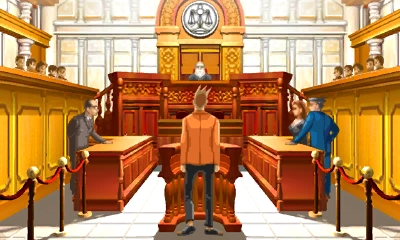
\includegraphics [width=10cm]{images/aa_screen_original.jpg}
	\caption{Un aperçu du jeu original}
	\label {screen_game}
\end{figure}
  \cleardoublepage
  \section{Raisons du projet}
	Dans cette partie nous allons détailler les raisons qui nous ont amenées à choisir ce sujet.\newline

\subsection{Une passion commune}

	Tout d'abord, nous sommes tous les deux des passionés de jeux vidéos et tout particulièrement de la série Ace Attorney. De ce fait, cela nous a paru comme une évidence de choisir cet univers et de vouloir le représenter en 3D. En effet, les jeux originaux sont en 2D et offre une variété graphique assez faible au niveau des détails sur la profondeur et des mouvements de caméra. Pouvoir recréer entièrement cet univers en utilisant la biliothèque OpenGL nous a donc offert une totale liberté de mouvement créant des angles de vue totalements inédits.
  \cleardoublepage
  \newpage
  \section{Les Fonctionalités Graphiques}

\subsection{Les Fonctions Utisant OpenGL}
	\subsubsection{Le sol}
	Le sol et constitué de 6 pavés mis côte à côte, afin d'avoir une plus belle réflexion de la lumière. Ces pavés sont eux même composés de sous pavés, qui ne sont au final que de simples GL\_QUADS, sur lesquels on plaque une texture de pavage à neuf cases.
	
	\subsubsection{Les meubles}
	Les meubles sont créer grâce à la fonction creer\_pave, qui prends en paramêtre les coordonées du centre du pavé, ainsi que sa largeur, sa profondeur et sa hauteur. Cette fonction crée correctement toutes les faces vers l'exterieur, et fixe leurs normales, afin que la lumière et les textures ajoutées s'affichent correctement.
	\subsubsection{Les murs}
	Les murs sont crées par la fonction creer\_mur, qui ressemble beaucoup à creer\_pave, mais ne crée pas les faces en z et -z, et qui de plus, crée les faces vers l'interieur du solide.
	\subsubsection{Le blason, et la balance}
	Les éléments situés au dessus du juge ont été crées à l'aide des fonctions de la glu, gluCylinder, et gluDisk. Elles sont tournées et translatées sur le fond de la pièce, et des texture réalistes sont plaquées dessus.
	\subsubsection{Le marteau et son support}
	Le marteau, tout comme les précédents éléments, est crée à l'aide d'un quadric, avec les fonctions de la glu. Il a aussi été ajouté un glRotatef dedans, afin de pouvoir faire varier la position du marteau. Cela simule un coup au rendu convainquant.
	\subsubsection{Le Stand des Témoins}
	Ce stand est constitué en bas d'un ensemble de pavés, créé par la fonction décrite si dessus, repartis de façon homogène sur un demi-cercle. Il est surmonté par des gluPartialDisk empilés les uns sur les autres.
	\subsubsection{Les personnages}
	Pour créer les personnages, une nouvelle fonction a due être definie, c'est la fonction creer\_pave\_with\_texture, cette fonction permet d'associer à chaques faces d'un pavé, une texture différente, fournie en argument de la fonction. De plus, certains personnages ont subit quelques modifications, permettant des animations, au grés du scénario.
	En effet, les bras du personnage principal sont affublés de deux glRotatef, ce qui leurs permet de bouger dans deux directions différentes, le bras du juge, à l'aide d'un glTranslatef, bouge au rythme de son marteau, et les têtes des spectateurs de la foule peuvent, à l aide d'un glRotatef, tourner de gauche à droite.
	\subsubsection{Les arcades}
	Des arcades ont été appliquées sur les murs afin d'améliorer leur esthétisme. Deux pavés créés normalement, surmontés de deux autres, qui sont tournés à 45 degrés et déplacés au dessus des premiers.
\subsection{Le modèle de vu}
	Afin d'afficher la scène, un gluPerspective est fait à l'initialisation. Les arguments associés sont un fovy de 60, ce qui nous a semblé rendre une scène correcte, non déformée. Le rapport d'aspect reste à 1, near est à 10 et far est à 3000 ce qui permet, quelque soit notre emplacement dans la scène, de pouvoir l'afficher en entier.\newline
	Un gluLookAt est fait à chaque fois que la scène est affichée, il prend en paramètre des variables globales ce qui permet de pouvoir facilement déplacer la camera dans la scène. Il y deux façons de se déplacer dans la scène.
	\subsubsection{Le mode "Vue libre"}
	Grâce à la fonction PollEvent de le SDL, on peut récupérer les inputs fait au clavier quand la fenêtre à le focus, cela permet de pouvoir modifier les globales whereiam{x,y,z} et whereialook{x,y,z} offrant une totale liberté de mouvement dans la scène.
	\subsubsection{Le mode automatique}
	Certaines touches, ou certaines balises dans le script, lancent les fonctions de déplacement, qui elles-mêmes appellent movecamera, qui permet de deplacer de manière fluide la camera dans la scène, en faisant un display de la scène tous les 1/100 ème de la distance entre où je suis et l'endroit où je dois être.
\subsection{Les animations}
	Plusieurs fonctions permettent de créer de petites animations, et sont lancées par des évements clavier créés manuellement ou par le biais du script. Ces fonctions modifient la valeur des variables globales mentionnées plus haut, et affichent la scène plusieurs fois afin de pouvoir voir l'animation complète.
\subsection{La musique}
	Grace à SDLmixer, de la musique à été ajoutée au projet, reprenant les sonorités classiques du jeu. Ces musiques sont jouées lors d'évènements de clavier, ou bien lors d'animations (comme par exemple celui du marteau qui est associé à son mouvement). Il y a deux types de musiques.
	\subsubsection{Les musiques standarts}
	Ce sont celles couramment jouées en fond sonore, pendant la lecture du script. Une seule peut être jouée à la fois, et certaines bouclent alors que d'autres ne sont jouées qu'une fois.
	\subsubsection{Les "morceaux" de musique}
	Ce sont les bruitages qui ne couperont pas la musique de fond quand ils seront joués. Ce sont principalement les objections des avocats, et autres interjections.
	
  \cleardoublepage
  \section{Les fonctionnalités du script}

	Le but de notre projet était de revisiter l'univers d'Ace Attorney et ce de deux manières différentes:
d'une part  grâce à la réalisation graphique, que nous verrons plus tard dans ce rapport, et d'autre part par le suivi du script.\newline

	En effet, comme dit en introduction, le script a une place majeure dans le déroulement du jeu car c'est lui qui fait avancer ou non l'intrigue.\newline
Pour des soucis de temps, nous avons choisi de ne ré-implémenter que la première affaire du premier jeu.\newline

	Cette partie du rapport se découpe de la manière suivante: dans un premier temps, nous verrons comment les différents fichiers de script s'organisent entre eux.Dans un second temps, nous décrirons les structures utilisées pour la bonne gestion des fichiers de textes selon la situation. Enfin, nous verrons comment l'implémentation de cette partie en elle même.\newline

\subsection{Les fichiers}
Tout d'abord, les fichiers de textes sont tous placés dans le dossier ./text\_files/ afin de bien séparer les morceaux de l'application finale.
Ces fichiers s'articulent donc en plusieurs catégories qui sont les suivantes:

\begin{itemize}
	\item evidences.txt -> ce fichier sert à lister toutes les preuves ainsi qu'une petite description de celles-ci
	\item script.txt -> le script général. C'est le fichier parent à tous les autres.
	\item qcms/ -> les différents qcms du script en cours
	\item cross\_exams/ -> les fichiers représentant la contre-argumentation en cours
	\item testimonies/ -> les différents témoignages du script en cours.
\end{itemize}

	Dans le fichier script.txt, et ceux qui en découlent, nous trouveront un certains nombre de balises, délimitées par "[" et "]", qui indiquent une certaine action à effectuer en fonction du contenu de la balise (que ce soit le lancement d'une musique ou d'une autre partie du script), sauf quand un personnage parle: cette information est indiquée par une "*" avant le nom du personnage, et les lignes de dialogues qui suivent sont affichées sur la console.


\subsection{Les structures}

	Dans cette partie, nous allons décrire les différentes structures associées à la gestion du script et à sa bonne exécution.

\begin{verbatim}

struct key_value {
	char *key;
	char *value;
};
\end{verbatim}

	Cette structure est la structure classique pour contenir un couple de clé-valeur.

\begin{verbatim}

struct qcm_struct {
	char *talking;
	char *question;
	char *answer[5];
	int nb_proposition;
	struct key_value proposition_case[5];
	char *case\_files[5];
};
\end{verbatim}

	La structure d'un QCM renseigne toutes les informations utiles à la progression de celui-ci, c'est à dire le personnage posant la question, la question en elle même, les réponses possibles, le nombre de propositions, un couple de clé/valeur associant comme clé "CASE\_i" à la valeur de texte qui sera affiché dans le menu du QCM. Enfin, la structure enregistre les différents fichiers qui seront lus quand une réponse est proposée.

\begin{verbatim}


struct evidence {
	char *evidence_name[30];
	char *evidence_type[30];
	char *evidence_other[30];
	char *evidence_description[30];
	int evidence_active[30];
	int nb_evidence;
};
\end{verbatim}

	Cette structure permet l'enregistrement des informations sur les preuves contenues dans le fichier "evidences.txt", avec notamment son nom, son type, sa description, si elle est active ou non et ses informations complémentaires. La structure renseigne également sur le nombre de preuves totales du fichier.

\begin{verbatim}

struct cross_exam_struct {
	char *answer_line[15];
	int evidence_to_show;
	char *lines[20];
	char *extras[20];
	char *name;
	int current_line;
	int nb_lines;
	int nb_extras;
};

\end{verbatim}

	Dernière structure de données permettant l'emcapsulation des informations pour le bon déroulement d'une contre-argumentation. Elle possède toutes les lignes du témoignage, les lignes correctes sur lesquelles on peut présenter une preuve et si le numéro de la preuve (evidence\_to\_show) est la bonne fini la contre-argumentation. Après avoir passé toutes les lignes du témoignage, on affiche les lignes "extras", c'est à dire, un petit dialogue qui se passe après mais qui en conclue pas cette phase de jeu.
	
\subsection{L'implémentation de la lecture du script}
	
	En premier lieu, pour éviter que la lecture du script n'empiète sur l'affichage de la scène, et donc pouvoir utilisé les différentes touches claviers pour effectuer les actions que nous avons définies, nous avons dû l'encapsuler dans un thread POSIX afin de vraiment dissocier le thread principal gérant l'affichage de la scène et le thread utilisateur permettant la lecture des différents fichiers.\newline
	
	Dans un second temps, dès qu'une ligne indiquant le changement de fichier (par les balises [QCM] ou [CROSS\_EXAM]), un nouveau fichier est lu, mettant en suspend la lecture en cours. Des fonctions sont prévues pour ces deux cas là, car ils sont différents d'une simple lecture puisqu'ils répondent à un certain gameplay.\newline
	
	Dans l'implémentation proposée, on vérifie également la ligne du script lue pour savoir le comportement a adopté. En effet, si la ligne commence par une étoile, on indique qu'il faut changer le point de vue de la caméra pour pointer sur le personnage qui parle.\newline
	Pour des balises de type [START\_MUSIC\_TRIAL] ou [JUDGE\_HAMMER] cela lance la musique ou bien la petite animation associée à ce type d'évènement.\newline
	
	Pour parvenir à indiquer à la partie graphique qu'un changement doit être opéré, et ce parce que les deux parties de l'application sont sur deux threads différents, nous avons dû nous servir de la fonction SDL\_PushEvent(SDL\_Event *event) permettant d'empiler sur la pile des évènements de la SDL pour que la partie graphique puisse se mettre à jour en fonction des données du script. Nous avons pu utiliser cette fonction puisque la documentation de la SDL indique que celle-ci est "thread-safe" et que les changements opérés sur un thread seront visibles sur un autre.
  \cleardoublepage
  \section{Autres}
	
	Dans cette partie, nous allons présenter les problèmes que nous avons rencontrés au cours de ce projet, les améliorations possibles pour pouvoir le continuer et enfin les compétences que nous avons acquise lors de la réalisation des différentes parties du projet.
	
\subsection{Problèmes rencontrés}
	Dans ce projet nous avons rencontré différentes difficultés. Tout d'abord, il a fallut s'initier à l'utilisation d'OpenGL. Certains aspects furent compliquer à réaliser, notamenent réussir une projection au bon endroit avec volume de vue adéquat. Mais aussi créer de solides avec des faces dans le bon sens, des textures corectement appliquées. Il nous a fallut aussi gerer l'éclairement, la décompositon de certains éléments en pavage pour un rendu plus lisse. La lumière diffuse a aussi été dûre à gérer, longtemps les faces opposées à la lumière sont restées noires. Il a aussi fallut gérer un grand nombre de textures, leur application dans le bon sens sur chaqu'unes des figures. De plus, il a fallut comprendre l'utilisation des quadriques et l'appliquation des textures sur eux. Le witness stand a requis l'usage formules de trigonometrie afin d'obtenir une disposition homogène des piliers.
	Du coté de la lecture du script, les complications ont été d'encapsuler les accès mémoire dans un thread, pour ne pas ralentir la fenetre graphique.
	 Enfin, il modularisation du programme en fichiers disjoints a été longue à faire à cause des étroits liens entre les globales et leurs initialisation, et leur usage dans des fonctions.
\subsection{Idées d'améliorations}
	Musiques manquantes
	Textures pas géniales
	Persos cubiques
	Mauvaise gestion de l'espace (gros vide)
	Pas de plafond 
	Continuer le jeu, si ce n'est le terminé (transition et autres affaires)
	Gestion sauvegarde/pénalité
	Mise en forme et nettoyage du code
	Créér nos prepres events
	Affichage des preuves

\subsection{Compétences acquises}
	Manipulation OpenGL
	Manipulation SDL -> File d'events
	Manipulation thread POSIX
	Manipulation Fichiers/Chaines de Caracteres
  \cleardoublepage
  \section*{Conclusion}
\addcontentsline{toc}{section}{Conclusion}

	Pour conclure, ce projet fut enrichissant en nous permettant de manipuler une bibliothèque capable de faire des scènes 3D avec un rendu très proche de ce que nous avions prévus de faire grâce aux gestions des textures et de la lumière.\newline 
	
	Il fut également enrichissant dans le fait que nous avons réutilisés nos connaissances en système pour pouvoir utilisé les threads POSIX et ainsi bien séparer la partie graphique de la partie lecture de fichiers.\newline
	
	Dans l'avenir, ce projet pourra être repris et étoffé pour en faire un moteur de ce type de jeu ou bien le reprendre comme base pour recréer entièrement le jeu dont s'est inspiré notre réalisation.


  \cleardoublepage
  \newpage
\begin{appendices}
\section{Lexique}
\begin{itemize}
	\item EDT~:
	EDT est un acronyme signifiant Event Dispatch Thread. Concrètement, EDT est le thread principal s'occupant de la partie graphique d'une application Java, c'est-à-dire le dessin de l'IHM ou la gestion des interactions avec l'utilisateur.
	\newline

	\item Itérateur~:
	En programmation, un itérateur est un objet permettant de parcourir un tableau ou une collection, non pas nécessairement depuis le début du tableau, mais depuis n'importe quel index du tableau. Dans le cadre de notre projet, notre itérateur nous permet de parcourir notre Board.
	\newline

	\item Pair à pair~:
    Le pair à  pair (ou peer-to-peer en anglais), est un modèle de réseau permettant à deux machines de discuter d'égale à égale.
    Dans les faits, cela s'explique par le fait qu'une machine se connecte à une autre machine et inversement afin que celles-ci puissent s'échanger des informations sans passer par un serveur distant.
    \newline
    
   	\item Protocole réseau~:
    Un protocole est une méthode standard qui permet la communication entre des processus (s'exécutant éventuellement sur différentes machines), c'est-à-dire un ensemble de règles et de procédures à respecter pour émettre et recevoir des données sur un réseau. 
    Il en existe plusieurs selon ce que l'on attend de la communication. Certains protocoles seront par exemple spécialisés dans l'échange de fichiers (le FTP), d'autres pourront servir à gérer simplement l'état de la transmission et des erreurs (c'est le cas du protocole ICMP), ... 
	\newline

	\item Protocole TCP~: 
    Acronyme de Transmission Control Protocol, le protocole TCP/IP est le protocole standard utilisé sur internet, pour la liaison entre deux ordinateurs.
    Le protocole TCP vérifie la validité des paquets après leur réception afin d'être sûr de la validité de celle-ci.
    Le protocole TCP est située sur la couche 4 (couche de transport) du modèle OSI. 
	\newline
	
	\item Protocole UDP~:
    Acronyme User Datagram Protocol, le protocole UDP est un des protocoles standards utilisé sur internet. 
    La différence avec TCP est que les paquets sont reçus sous forme de datagrammes qui doivent être vérifiés pour valider la qualité du paquet reçu.
    Le protocole UDP est très utilisé, notamment, dans le cadre du jeu en ligne, ou encore le streaming, car la perte de paquet influe peu sur la quantité reçus.
    Le protocole UDP est située sur la couche 4 (couche de transport) du modèle OSI, au même titre que le protocole TCP. 
   \newline

	\item Socket~:
    Une socket est une interface de connexion bidirectionnelle permettant l'échange de données entre deux processus (distants ou non).
	\newline
 
	\item Socket de Berkeley~:
    Les sockets de Berkeley, sont un ensemble normalisés de fonctions de communications lancé par l'université de Berkeley au début des années 1980.
    De nos jours, elle est la norme utilisé par quasiment l'ensemble des langages de développement (C, Java, Python, ...).
    \newline
  
	\item Socket d'écoute~:
    Une socket d'écoute est une socket présente uniquement dans le protocole TCP. En effet, son rôle consiste, comme son nom l'indique, à écouter les demandes de connexion de socket externe sur un port prédéfini, afin de créer une socket qui permettra ensuite l'échange de données avant de reprendre son rôle d'écouteur.
	\newline
  
	\item Socket de service~:
    La socket de service est la socket crée par la socket d'écoute lorsque celle-ci reçoit une demande de connexion. La socket de service permet la communication entre le serveur et le client ayant fait une demande de connexion. C'est par cette socket que transitent toutes les données émises par le client et le serveur.
	\newline
  
	\item Thread~:
	Un thread est une sorte de processus, dit "léger". Le rôle d'un thread est d'exécuter une suite d'instruction précise que l'on peut nomme routine.
	Le fait de lancer une application informatique lance automatiquement un thread, celui-ci peut alors créer d'autres threads afin de délégué par exemple une tâche longue a un autre thread, afin que le thread principal (main thread), puisse continuer son fil d'exécution à lui.
	\newline

   
\end{itemize}


\newpage
\section{Webographie}
\begin{itemize}
	\item Fonctionnement des intelligences artificielles~: \url{http://www.datagenetics.com/blog/december32011/index.html}
\newline	
	\item API Java~: \url{https://docs.oracle.com/javase/7/docs/api/}
	\newline
	\item Règles de la bataille navale: \url{http://www.regles-de-jeux.com/regle-de-la-bataille-navale/}
\end{itemize}

\newpage


\end{appendices}

\end{document}

